\appendix

\section{Calibration targets}
\label{app:targets}

This study calibrates to the full materialized target surface \populace{} currently constructs for the
US fiscal build. Every target is a source-backed fact from PolicyEngine Ledger \citep{ledger2026}, the
\texttt{arch-data} fact store that holds the source publications and preserves the provenance of each
published value; Populace composes calibration targets from those facts. The surface combines national,
state, and congressional-district aggregates across the major tax and transfer families
(Table~\ref{tab:target_sources}). It is reported here in full so the empirical claims can be read against
the exact target system used rather than against a pipeline-wide inventory.

Table~\ref{tab:target_sources} lists each family with its administrative source. The system holds
31{,}534 targets across eleven families and three geographic levels: 23{,}450 congressional-district,
7{,}615 state, and 469 national targets. The \texttt{irs\_soi} family supplies 30{,}252 of them (96\%),
so the micro-average over all targets is dominated by IRS income-tax aggregates; the family
macro-average (Section~\ref{sec:metrics}) is the counterweight that gives each family equal weight.

\begin{table}[H]
\centering
{\tablefont
\begin{tabular}{@{}p{0.24\textwidth}p{0.40\textwidth}p{0.13\textwidth}r@{}}
\toprule
Family & Administrative source & Levels & Targets \\
\midrule
\texttt{irs\_soi} & IRS Statistics of Income: Historic Table 2 state totals and congressional-district tables & National, state, district & 30{,}252 \\
\texttt{census\_population} & Census Bureau annual state resident population estimates & National, state & 936 \\
\texttt{cms\_medicaid} & CMS Medicaid and CHIP applications, eligibility, and enrollment reports & National, state & 102 \\
\texttt{cms\_aca} & CMS open-enrollment-period state-level public use file & State & 102 \\
\texttt{usda\_snap} & USDA FNS SNAP monthly state participation and benefit summaries & National, state & 52 \\
\texttt{state\_income\_tax} & Census Bureau State Tax Collections (STC), item T40 individual income taxes & State & 44 \\
\texttt{hhs\_acf\_tanf} & HHS ACF federal TANF and state MOE financial data & National, state & 30 \\
\texttt{ssa} & SSA Annual Statistical Supplement, OASDI beneficiaries and benefits & National & 6 \\
\texttt{jct} & JCT estimates of federal tax expenditures & National & 5 \\
\texttt{cbo} & CBO revenue projections by category & National & 4 \\
\texttt{cms\_medicare} & CMS Medicare Trustees Report & National & 1 \\
\midrule
\textbf{Total} & & & \textbf{31{,}534} \\
\bottomrule
\end{tabular}
}
\caption{Calibration target families and their administrative sources. Counts and sources are read from
the full-surface target registry used by the run. In the headline experiment all listed families are fit
and scored; holdout variants are supplemental diagnostics (Section~\ref{sec:oos}).}
\label{tab:target_sources}
\end{table}

\section{From a record budget to the sparsity penalty}
\label{app:presets}

The sparsity penalty $\lambda_{L_0}$ sets the retained-record count, but the map from a penalty to a
count is monotone and problem-dependent rather than closed-form: a larger $\lambda_{L_0}$ prunes more
records, and how many depends on the candidate universe and the targets. Each build therefore specifies
a requested record count, and an outer bisection adjusts $\lambda_{L_0}$ over eight steps (each a full
optimization) until the achieved count matches. Table~\ref{tab:presets} reports the $\lambda_{L_0}$ that
each requested count converged to (informed $L_0$, $\lambda_{L_2}=0$), with the achieved count. The penalty
spans about an order of magnitude across the budget range, and the achieved count lands within three per
cent of the request at every point.

\begin{table}[H]
\centering
{\tablefont
\begin{tabular}{rrr}
\toprule
Requested records & $\lambda_{L_0}$ (converged) & Achieved records \\
\midrule
2{,}000  & $4.9\times10^{-5}$ & 1{,}962 \\
5{,}000  & $2.3\times10^{-5}$ & 4{,}935 \\
10{,}000 & $1.2\times10^{-5}$ & 9{,}770 \\
20{,}000 & $5.0\times10^{-6}$ & 20{,}406 \\
40{,}000 & $2.1\times10^{-6}$ & 39{,}586 \\
\bottomrule
\end{tabular}
}
\caption{The sparsity penalty $\lambda_{L_0}$ that each requested record count converged to under the
eight-step budget bisection (\texttt{weighted-loss-3seed}, informed $L_0$, $\lambda_{L_2}=0$), with the
achieved retained-record count. Values are means over three seeds. A larger $\lambda_{L_0}$ prunes more
records; the bisection sets it per build rather than by hand.}
\label{tab:presets}
\tablenote{$\lambda_{L_0}$ and the achieved count are read from each run's metrics; the achieved count is
within three per cent of the requested count at every budget.}
\end{table}


\section{Optimization hyperparameters}
\label{app:hyperparameters}

Table~\ref{tab:hyperparameters_full} lists the hyperparameters of the $L_0$ optimization with their
roles. The gate parameters follow the Hard Concrete construction of \citet{louizos2018}. The
sparsity penalty $\lambda_{L_0}$ and the epoch count are set per build to reach a target dataset
size and are reported with each run.

\begin{table}[H]
\centering
{\tablefont
\begin{tabular}{@{}l l p{0.46\textwidth}@{}}
\toprule
Parameter & Value & Role \\
\midrule
Gate temperature $\beta$ & 0.25 & Sharpness of the 0/1 gate transition \\
Left stretch $\gamma$ & $-0.1$ & Enables exact-zero gates after clipping \\
Right stretch $\zeta$ & 1.1 & Enables exact-one gates after clipping \\
Initial keep probability & 0.8 & Records start mostly active while leaving room for the sparsity penalty to close gates \\
Weight jitter SD & 0.05 & Log-space noise on weights at initialization \\
Logit jitter SD & 0.01 & Log-space noise on gate logits at initialization \\
Learning rate & 0.02 & Adam optimizer step size \\
Epochs & 250 & Training iterations per bisection step \\
Target loss cap $c$ & 1 & Caps a single target's contribution to $\mathcal{L}_{\text{cal}}$; the runs reported here use Populace's production US-fiscal value $c=1$ \\
$\lambda_{L_0}$ & $5.9\times10^{-3}$ to $1.4\times10^{-2}$ & Sparsity penalty, set per build by bisection to the target size (Appendix~\ref{app:presets}) \\
$\lambda_{L_2}$ & $0$ & Soft concentration penalty on $(w_i/w_{0,i})^2$ (mean over records); held at zero in the reported full-surface run \\
Budget bisection steps & 8 & Re-runs of the optimization that tune $\lambda_{L_0}$ to the target size \\
\texttt{max\_weight\_ratio} & None (uncapped) & Hard per-record weight cap: $w_i \leq \text{ratio}\times w_{0,i}$, clamped each step \\
\bottomrule
\end{tabular}
}
\caption{Hyperparameters for the $L_0$ optimization. Gate parameters follow \citet{louizos2018}.
Source: the \texttt{l0-python} Hard Concrete implementation used by \populace{}.}
\label{tab:hyperparameters_full}
\end{table}

\section{Algorithm pseudocode}
\label{app:algorithm}

Algorithm~\ref{alg:l0} presents the $L_0$-regularized calibration procedure.

\begin{algorithm}[H]
\caption{$L_0$-regularized calibration with Hard Concrete gates}
\label{alg:l0}
\begin{algorithmic}[1]
\Require Calibration matrix $\mathbf{M} \in \R^{m \times n}$, targets $\mathbf{t} \in \R^m$, initial weights $\mathbf{w}_0 \in \R^n$, per-target loss weights $\boldsymbol{\omega} \in \R^m$
\Require Hyperparameters: $\lambda_{L_0}$, $\lambda_{L_2}$, weight cap $r$ (\texttt{max\_weight\_ratio}; $\infty$ if uncapped), $\beta$, $\gamma$, $\zeta$, learning rate $\eta$, epochs $E$
\Ensure Calibrated sparse weight vector $\hat{\mathbf{w}} \in \R^n$

\State Initialize $\log w_i \gets \log w_{0,i} + \mathcal{N}(0, 0.05^2)$ for all $i$
\State Initialize $\log \alpha_i \gets \text{logit}(0.8) + \mathcal{N}(0, 0.01^2)$ for all $i$
\State Initialize Adam optimizer with parameters $\{\log w_i, \log \alpha_i\}$ and learning rate $\eta$

\For{epoch $= 1$ to $E$}
    \State \textbf{Sample Hard Concrete gates (training):}
    \For{$i = 1$ to $n$}
        \State $u_i \sim \text{Uniform}(\epsilon, 1-\epsilon)$
        \State $s_i \gets \sigma\!\left(\frac{\log u_i - \log(1-u_i) + \log \alpha_i}{\beta}\right)$
        \State $\bar{s}_i \gets s_i(\zeta - \gamma) + \gamma$
        \State $z_i \gets \min(1, \max(0, \bar{s}_i))$
    \EndFor
    \State $w_i^{\text{eff}} \gets \exp(\log w_i) \cdot z_i$ for all $i$
    \State $\hat{t}_j \gets \sum_i M_{ji} \cdot w_i^{\text{eff}}$ for all $j$
    \State $\mathcal{L}_{\text{cal}} \gets \dfrac{\sum_{j=1}^{m}\omega_j\,\min\!\left(\left|\frac{\hat{t}_j - t_j}{s_j}\right|, c\right)}{\sum_{j=1}^{m}\omega_j}$
    \State $\mathcal{L}_{L_0} \gets \sum_{i=1}^{n} \sigma\!\left(\log \alpha_i - \beta \log \frac{-\gamma}{\zeta}\right)$
    \State $\mathcal{L}_{L_2} \gets \frac{1}{n}\sum_{i=1}^{n}\left(\frac{\exp(\log w_i)}{w_{0,i}}\right)^2$ \Comment{soft concentration; informed $L_0$ only}
    \State $\mathcal{L} \gets \mathcal{L}_{\text{cal}} + \lambda_{L_0} \mathcal{L}_{L_0} + \lambda_{L_2} \mathcal{L}_{L_2}$
    \State Backpropagate $\nabla_{\log w, \log \alpha} \mathcal{L}$
    \State Adam step
    \State Clamp $\log w_i \gets \min\!\left(\log w_i,\; \log(r \cdot w_{0,i})\right)$ for all $i$ \Comment{per-record cap; no-op if $r=\infty$}
\EndFor

\State \textbf{Deterministic inference:}
\For{$i = 1$ to $n$}
    \State $z_i^{\text{det}} \gets \min\!\left(1, \max\!\left(0,\; \sigma(\log \alpha_i)(\zeta - \gamma) + \gamma\right)\right)$
    \State $\hat{w}_i \gets \exp(\log w_i) \cdot z_i^{\text{det}}$
\EndFor
\State \Return $\hat{\mathbf{w}}$
\end{algorithmic}
\end{algorithm}

\section{Dataset assembly details}
\label{app:assembly}

After optimization the fitted weight vector is mapped back to record form and used to assemble the
deployable dataset. The assembly step keeps the active records, reconstructs their person and
tax-unit memberships, derives geography from the stored assignment, and recomputes
geography-dependent quantities. Two details matter for fidelity. Geography is derived from the same
assignment used to build the calibration matrix, so the assembled dataset matches the universe the
optimizer saw. Take-up draws are regenerated with the same deterministic seeds used during matrix
construction, so take-up-dependent targets stay consistent between the calibration problem and the
assembled dataset.

\section{Cost diagnostics}
\label{app:cost}

Figure~\ref{fig:cost_accuracy} reports the wall-clock runtime of each method against the full-surface
median ARE it reaches, across the budget sweep, so the accuracy comparison can be read alongside its
compute cost.

\begin{figure}[H]
    \centering
    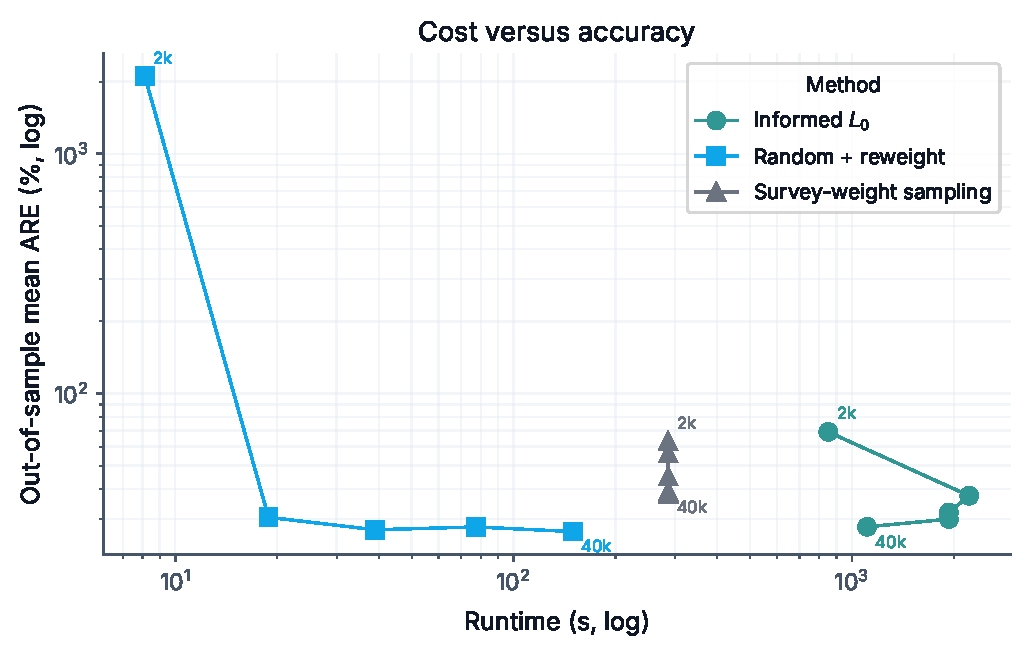
\includegraphics[width=0.8\textwidth]{figures/f5_cost_accuracy}
    \caption{Cost against accuracy: wall-clock runtime (log scale) against full-surface median ARE (log
    scale) for the four methods, each point labelled by its requested record budget. Informed $L_0$ and
    informed $L_0$ plus refit runtimes include the eight-step budget bisection that sets the sparsity
    penalty; the matched baselines run once at the budget. Points are the mean over three seeds.}
    \label{fig:cost_accuracy}
\end{figure}
